%ref: ципенюк, 96
{\footnotesize
  \textsc{Справка.} \emph{Дифференциальным сечением рассеяния} называется
  отношение числа частиц, рассеянных за единицу времени в элемент телесного угла
  $ d\Omega = \sin\theta\,d\varphi d\theta $, к плотности потока падающих частиц
  $ nv $, где $ n $ есть плотность частиц, а $ v $ --- их скорость. 

  \emph{Классическая модель Томпсона}. Требовалось объяснить нейтральность атома,
  несмотря на присутствие электронов. В этой модели электроны свободно плавают в некотором
  равномерно положительно заряженном облаке. Они не могут вылететь наружу, поскольку
  снаружи меньше положительного заряда, чем внутри.

  При распаде некоторых радиоактивных веществ испускаются \emph{$ \alpha
  $-частицы} --- положительно заряженные частицы, образованные двумя протонами и
  двумя нейтронами; ядро атома гелия.
}



Размышления основаны на классической физике. От радиоактивного источника $ \alpha $-частицы пропускались через узкое
отверстие, после чего пучок попадал на фотопластинку и давал на ней чёткое
изображение щели. Было замечено, что происходит \emph{рассеивание\footnote{То
  есть отдельные $ \alpha $-частицы отклоняются в движении.} $ \alpha
$-частиц}, то есть размытие полученного изображения, если заполнить место
проведения опыта --- вакуумную стеклянную полость --- газом. 

Даже для небольшого отклонения $ \alpha $-частицы потребовалась бы большая сила,
которой было неоткуда взяться в электрически нейтральной в среднем модели
Томпсона. 

Ученики Резерфорда поставили на пути пучка тонкую фольгу. Ими было обнаружено,
что угол отклонения $ \alpha $-частицы может (в одном случае из 8000 для
платиновой фольги) достигать величины,
близкой к $ 180^\circ $. Такое отклонение имеет вероятность
порядка $ 10^{-3500} $, если предположить многократное рассеивание в модели
Томпсона. Поскольку сильный эффект наблюдался редко, было предположено, что основную часть атома занимает пустота, а в
малом объёме находится массивное \emph{ядро атома}, а частица отклоняется
вследствие одного взаимодействия с этим ядром, чья масса много больше массы
$ \alpha $-частицы.

Будем рассматривать движение частицы относительно неподвижного массивного
центра. Её траекторией тогда будет гипербола (сочтём этот факт известным) с фокусом $ M $ (см. рисунок
\ref{fig:reser1}).
\begin{wrapfigure}{l}{0.4\textwidth}
	\centering
	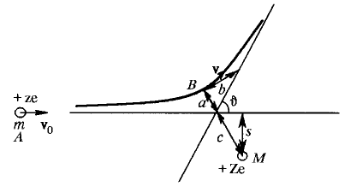
\includegraphics[width=0.4\textwidth]{img/oral-05/reser1.png}
  \caption{}
  \label{fig:reser1}
\end{wrapfigure}
Законы сохранения энергии и момента количества движения, если частица $ m $
последовательно находится в положениях $ A $ и $ B $, и закон Кулона непосредственно дают 
\begin{align*}
  \frac{1}{2} mv_0^2 &= \frac{1}{2}mv^2 + \frac{zZe^2}{a+c},\\
    mv_0s&=mv(a+c).
\end{align*}
На основании свойств гиперболы имеем\footnote{Из свойства гиперболы $ c^2 = a^2
  + b^2$, что влечёт равенство соответствующих треугольников и остальные два
соотношения.}
\begin{gather*}
    s = b, \quad c^2=a^2+b^2, \quad \tg \frac{\vartheta}{2} = \frac{a}{b},\\
    \tg \frac{\vartheta}{2} = \frac{zZe^2}{smv_0^2}.
\end{gather*}
\begin{wrapfigure}{r}{0.4\textwidth}
	\centering
	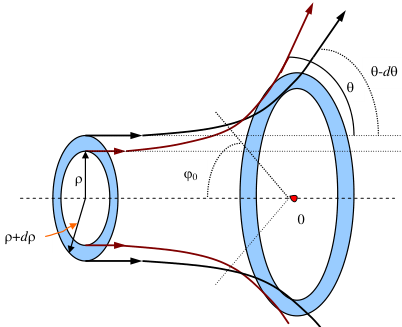
\includegraphics[width=0.4\textwidth]{img/oral-05/reser2.png}
  \caption{Рассеяние частиц с прицельным расстоянием $ \rho $.}
  \label{fig:reser2}
\end{wrapfigure}
Отсюда видно, что все частицы, попадающие в круговой слой $s $ и
$s + ds$, будут рассеиваться в угловом интервале $ \vartheta, \vartheta+d\vartheta $. Это
означает, что выделенная у ядра-мишени поверхность $ 2\pi s\,ds $ является
\emph{дифференциально эффективным сечением $ d\sigma $}. Поэтому с учётом  
\[
    |ds| = \frac{zZe^2}{mv_0^2}
    \frac{1}{\sin^2(\vartheta/2)}\frac{1}{2}\,d\vartheta
\]
мы получаем 
\[
    d\sigma = 2\pi \left( \frac{zZe^2}{mv_0^2} \right)^2
    \frac{1}{2}\frac{d\vartheta}{\tg(\vartheta/2) \sin^2 (\vartheta/2)}.
\]
Учитывая, что $ d\Omega = 2\pi\sin\vartheta\,d\vartheta $, мы окончательно
получаем 
\[
    d\sigma = \left( \frac{zZe^2}{2mv_0^2} \right)^2
    \frac{d\Omega}{\sin^4(\vartheta/2)}.
\]
Это и есть \emph{формула Резерфорда}. Отклонения от неё наблюдаются только для
очень малых углов рассеяния и для углов, близких к $ \pi $. Вскоре было
установлено, что электрический заряд центрального ядра в точности равен
номеру данного элемента в периодической таблице Менделеева.
Размер ядра $ \approx 10^{-12} $\,см, а размер орбиты\footnote{Позже выяснилось,
что никаких орбит не существует.} электронов $ \approx 10^{-8} $\,см.

\textsc{Несоответствие классической модели.} Летая по орбите, электрон имеет
ускорение. Значит, он должен выпускать световые волны и терять свою энергию. В
конце концов он должен был бы упать на ядро атома.




